\documentclass[25pt, a0paper, portrait, margin=0mm, innermargin=15mm, blockverticalspace=15mm, colspace=15mm, subcolspace=8mm]{tikzposter}
\usepackage{mathtools}
\usepackage{algorithm}
\usepackage{algorithmic}
\usepackage{wrapfig}
\usepackage{pgfplots}
\usepackage{subcaption}
\usepackage{etoolbox}
\usepackage{booktabs}

\title{Uncertainty propagation in neural networks for sparse coding}   \institute{University of Sheffield, UK, University of Oxford, UK }
\author{Danil Kuzin, Olga Isupova, Lyudmila Mihaylova}   \titlegraphic{Logo}
\usetheme{Autumn}
\usecolorstyle{Britain}
\begin{document}
  \maketitle
  \begin{columns}
    \column{0.5}
    \block{1-LISTA}{
      \innerblock{Sparse coding}{
        Reconstruct $\boldsymbol\beta$ from observations $\mathbf{y}$ collected as $\mathbf{y} = \mathbf{X} \boldsymbol\beta + \boldsymbol\varepsilon$, such that elements $\boldsymbol\beta$ contain zeros. 
      }
      \innerblock{LISTA}{
        \begin{itemize}
          \item Represent iterative soft-thresholding algorithm as a recurrent neural network with shared weights
          \item Learn weights with backpropagation through time
          \item Overfitting
          \item No uncertainty estimation
        \end{itemize} 

        \begin{algorithmic}[1]
          \REQUIRE observation $\mathbf{y}$, current weights $\mathbf{W}, \mathbf{S}$, number of layers $L$
          \STATE \textit{Initialisation.} Dense layer $\mathbf{b} \gets \mathbf{W}\mathbf{y}$
          \STATE \textit{Initialisation.} Soft-thresholding nonlinearity $\widehat{\boldsymbol\beta}_0 \gets h_\lambda(\mathbf{b})$
          \FOR{$l=1$ \TO $L$}
          \STATE Dense layer $\mathbf{c}_l \gets \mathbf{b} + \mathbf{S}\widehat{\boldsymbol\beta}_{l-1}$
          \STATE Soft-thresholding nonlinearity $\widehat{\boldsymbol\beta}_{l} \gets h_\lambda(\mathbf{c}_l)$
          \ENDFOR
          \RETURN $\widehat{\boldsymbol\beta} \gets \widehat{\boldsymbol\beta}_{L}$
        \end{algorithmic}     
      }
    }
    \block{3-Uncertainty propagation}{
      \innerblock{Idea}{
        At every step the output of soft-thresholding can be closely approximated with spike and slab distribution
      \begin{enumerate}
        \item \(\mathbf{b} = \mathbf{W}\mathbf{y}\) is Gaussian-distributed
        \item \(\widehat{\boldsymbol\beta}_{0} = h_\lambda(\mathbf{b})\) is approximated with the spike and slab distribution
        \item \(\mathbf{e}_l = \mathbf{S}\widehat{\boldsymbol\beta}_{l-1}\) is approximated with the Gaussian distribution
        \item \(\mathbf{c}_l = \mathbf{b} + \mathbf{e}_l\) is Gaussian-distributed
        \item \(\widehat{\boldsymbol\beta}_{l} = h_\lambda(\mathbf{c}_l)\) is approximated with the spike and slab distribution
      \end{enumerate}
      }
      \innerblock{Advantages}{
        \begin{itemize}
          \item All latent variables are modelled with parametrised distributions
          \item We can apply approximate Bayesian inference methods
        \end{itemize}
      }
    }
    \column{0.5}
    \block{2-BayesLISTA}{ 
      \innerblock{Bayesian LISTA}{
      \begin{itemize}
        \item Add priors for NN weights
        \item Perform full Bayesian inference
        \item Estimate uncertainty of predictions
      \end{itemize}
      }
    }
    \block{4-BackProp-PBP}{Blocktext}
    \block{5-Results}{
      \innerblock{Synthetic Experiments}{
        \begin{tikzfigure}[Different depth performance]
          \subcaptionbox*{\emph{NMSE}}{%
                     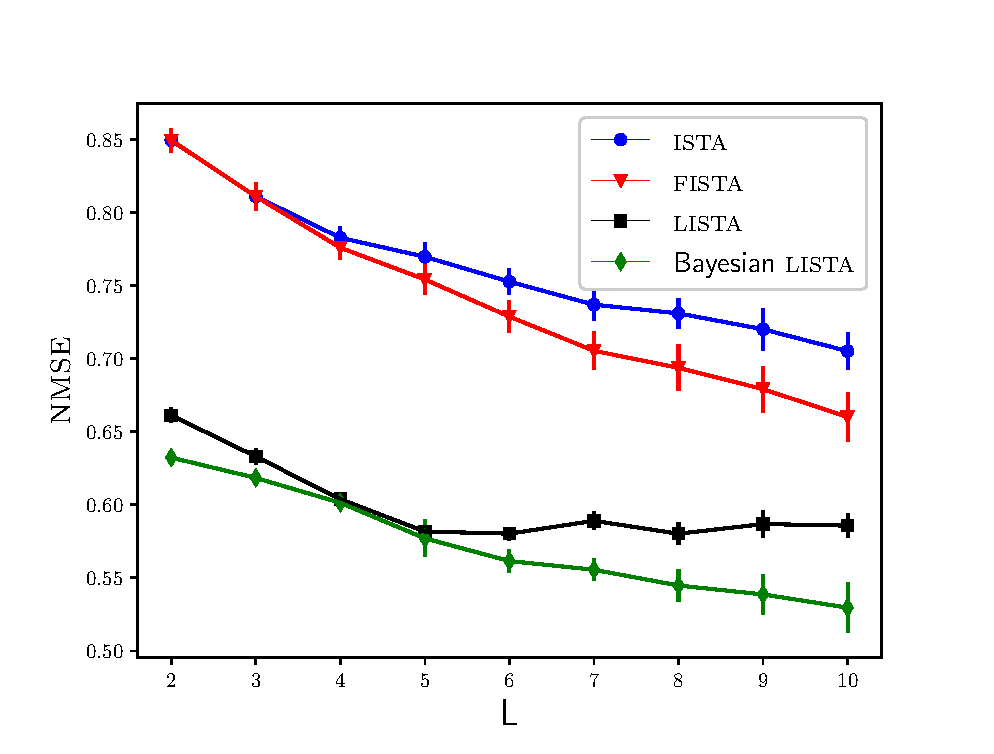
\includegraphics[width=200pt]{graphics/synthetic_number_of_layers/nmse_validation}
          }
          \quad
          \subcaptionbox*{\emph{F measure}}{%
                     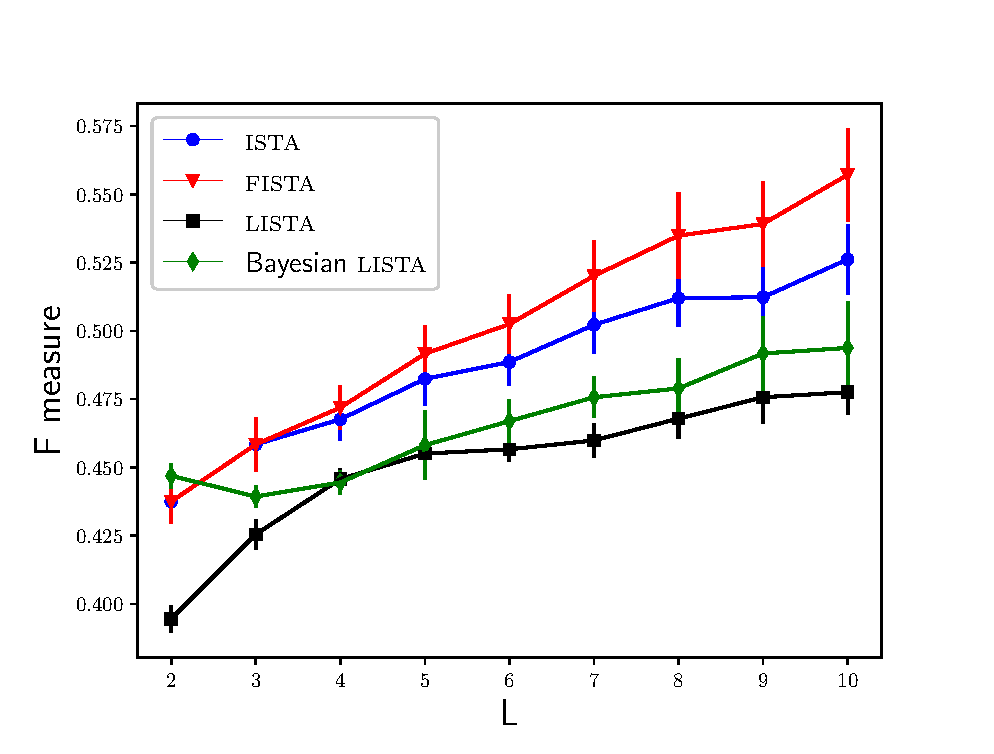
\includegraphics[width=200pt]{graphics/synthetic_number_of_layers/f_measure_validation}
          }
          %\captionsetup{labelformat=empty}
        \end{tikzfigure}

        \begin{tikzfigure}[Different observation size performance]
          \subcaptionbox*{\emph{NMSE}}{%
                     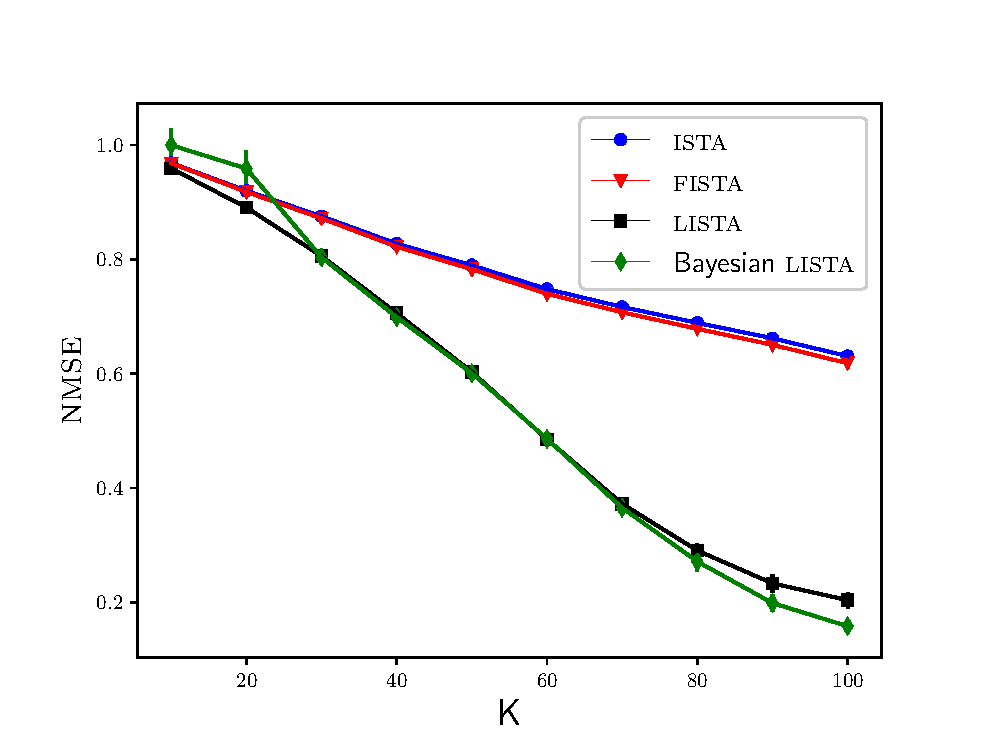
\includegraphics[width=200pt]{graphics/synthetic_undersampling/nmse_validation}
          }
          \quad
          \subcaptionbox*{\emph{F measure}}{%
                     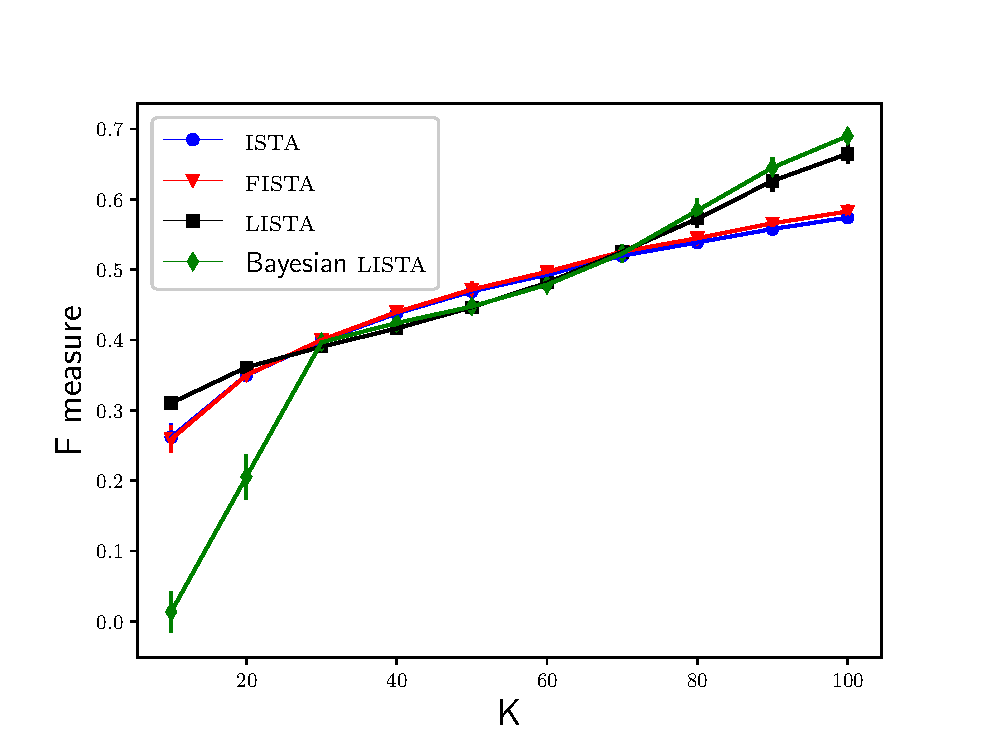
\includegraphics[width=200pt]{graphics/synthetic_undersampling/f_measure_validation}
          }
          %\captionsetup{labelformat=empty}
        \end{tikzfigure}
      }
      
      \innerblock{MNIST Experiments}{
        \begin{tikzfigure}[Posterior parameters for an image of digit 7]
          \subcaptionbox*{posterior mean}{
            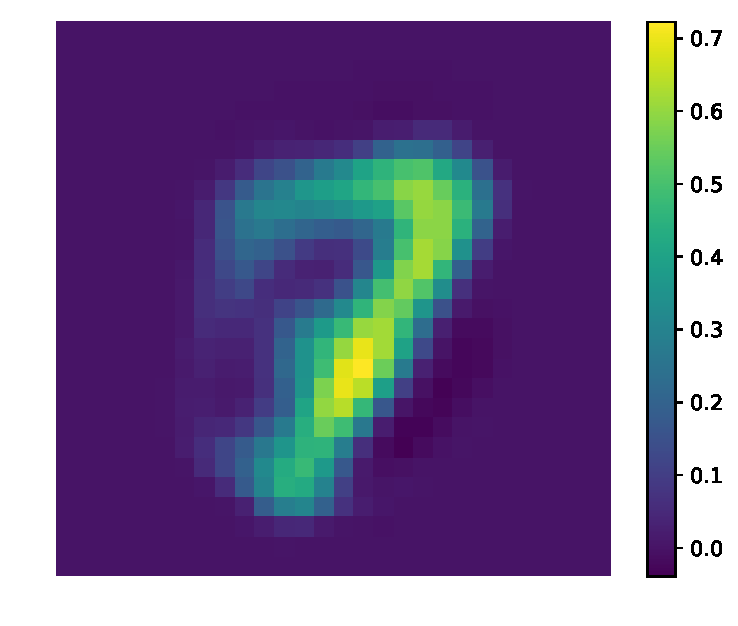
\includegraphics[width=200pt]{graphics/posterior_mean}
          }
          \quad
          \subcaptionbox*{posterior spike indicator}{
            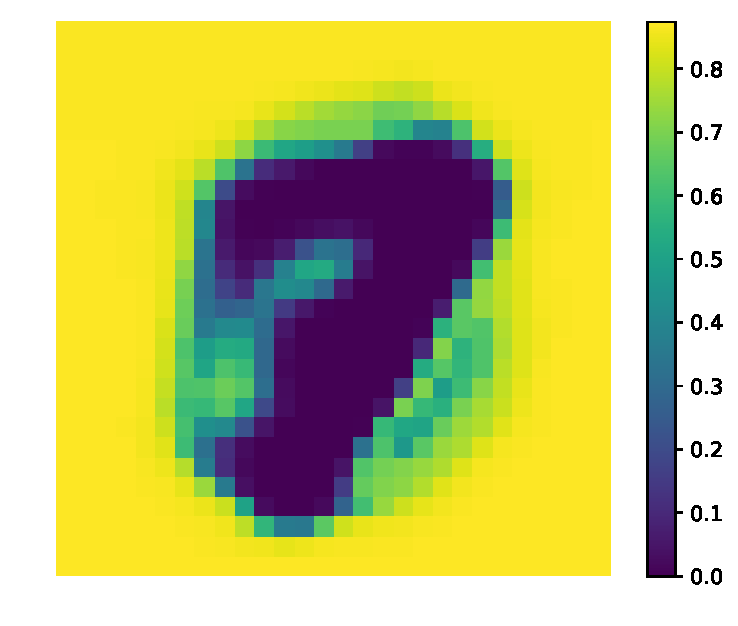
\includegraphics[width=200pt]{graphics/posterior_spike_indicator}
          }
        \end{tikzfigure}

        \begin{tikzfigure}[Samples from the posterior for an image of digit 7]
          \subcaptionbox*{posterior sample 0}{
            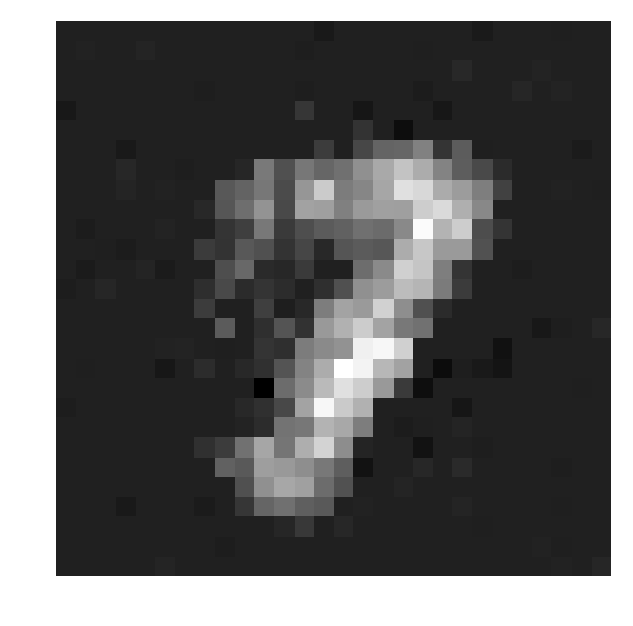
\includegraphics[width=150pt]{graphics/posterior_sample_0}
          }
          \quad
          \subcaptionbox*{posterior sample 1}{
            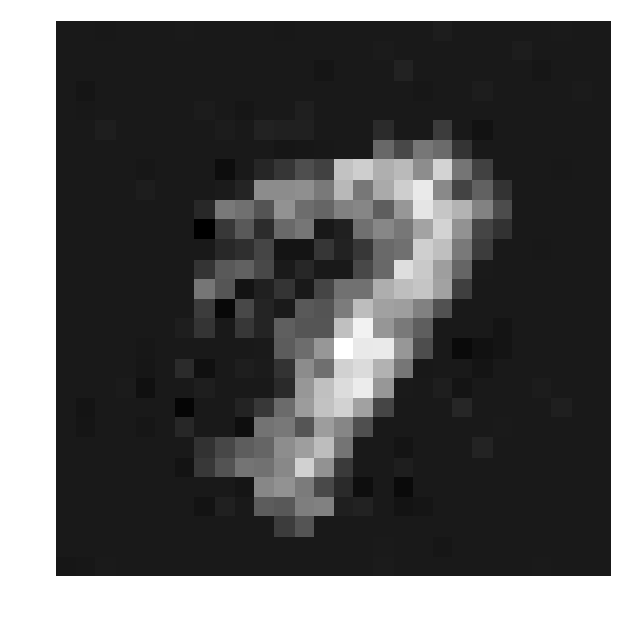
\includegraphics[width=150pt]{graphics/posterior_sample_1}
          }
          \quad
          \subcaptionbox*{posterior sample 2}{
            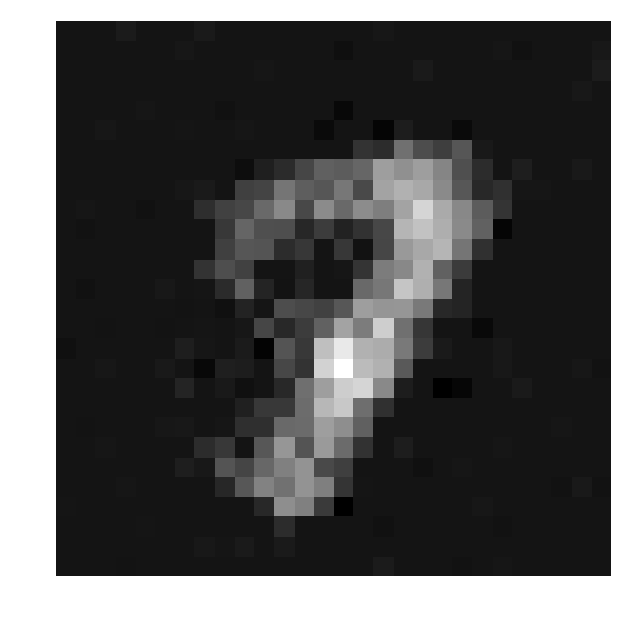
\includegraphics[width=150pt]{graphics/posterior_sample_2}
          }
        \end{tikzfigure}
      }
      
      \innerblock{Active Learning}{
        Use the estimated uncertainty to choose next training data with largest variance
        \begin{tikzfigure}[Sequential pool additions]
        \subcaptionbox*{NMSE}{
            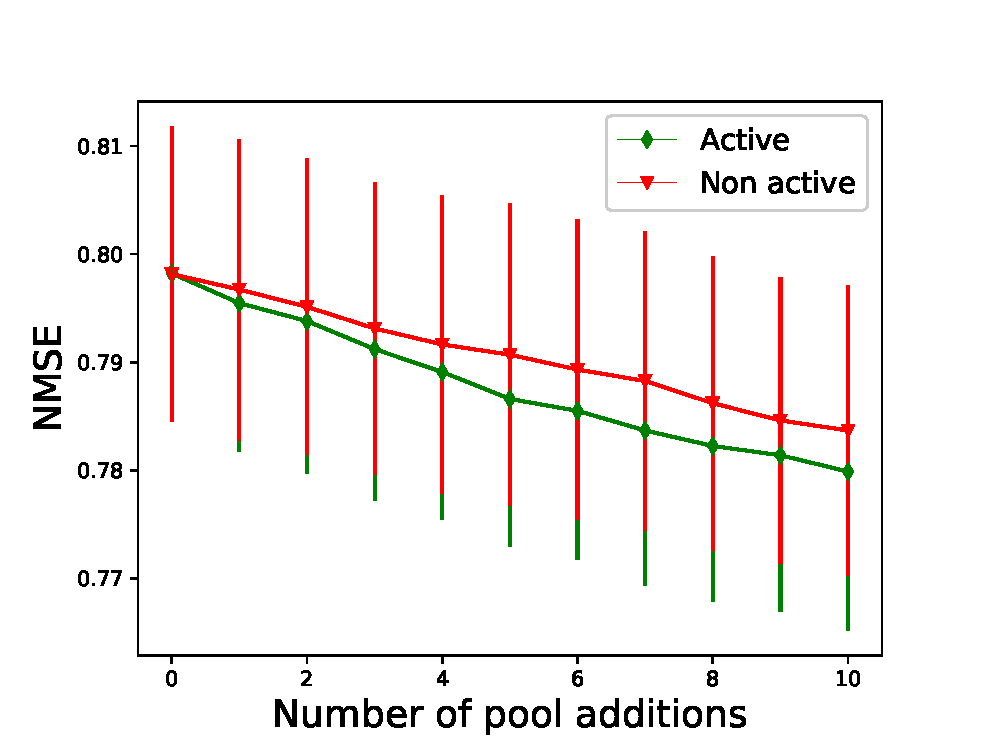
\includegraphics[width=200pt]{graphics/active_mnist/nmse_validation}
        }
        \subcaptionbox*{F measure}{
            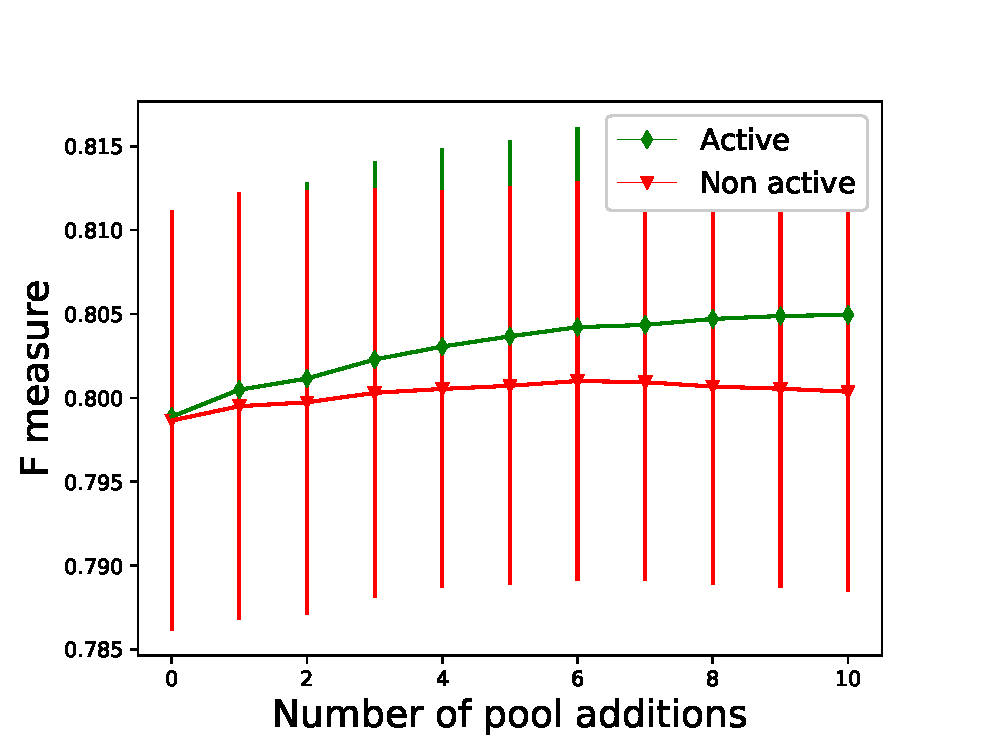
\includegraphics[width=200pt]{graphics/active_mnist/f_measure_validation}
        }
        \end{tikzfigure}
      }
    }
    
    \block{6-Summary}{Blocktext}
    \note{Notetext}
  \end{columns}
\end{document}
